% Springer Nature manuscript draft for PATTERN-Surv-HN
% Updated 21 September 2026 with aggregate-derived main and Extended Data figures.
% Match the author-provided architecture PDF's PDF 1.7 version to avoid an inclusion warning.
\pdfminorversion=7
\documentclass[pdflatex,sn-nature]{sn-jnl}
\usepackage{graphicx,multirow,amsmath,amssymb,amsfonts,xcolor,booktabs,array,tabularx,makecell,enumitem,url,float,placeins}
\definecolor{draftred}{RGB}{170,25,25}
\definecolor{softblue}{RGB}{232,241,250}
\newcommand{\TBD}[1]{\textcolor{draftred}{\textbf{[TBD: #1]}}}
\newcommand{\methodname}{PATTERN-Surv-HN}
\newcommand{\placeholderbox}[2]{\fbox{\begin{minipage}[c][#2][c]{0.94\textwidth}\centering\small\textbf{Figure framework placeholder}\\[6pt]#1\end{minipage}}}
\hypersetup{hypertexnames=false}
\raggedbottom
\begin{document}
\title[Clinically anchored multimodal survival prediction]{Clinically anchored multimodal survival prediction under missing, shifted and shortcut-prone evidence in head and neck cancer}
\author*[1]{\fnm{First} \sur{Author}}\email{corresponding.author@institution.edu}
\author[1]{\fnm{Second} \sur{Author}}
\author[2]{\fnm{Third} \sur{Author}}
\affil*[1]{\orgdiv{Department of \TBD{department}}, \orgname{\TBD{institution}}, \orgaddress{\city{\TBD{city}}, \country{\TBD{country}}}}
\affil[2]{\orgdiv{Department of \TBD{department}}, \orgname{\TBD{institution}}, \orgaddress{\city{\TBD{city}}, \country{\TBD{country}}}}
\abstract{Multimodal prognostic models are often developed as though every recorded modality were simultaneously available and equally trustworthy. We developed PATTERN-Surv-HN, a clinically anchored framework for postoperative head and neck squamous cell carcinoma survival prediction in which usable blood, ICD and tissue-microarray measurements contribute only as a shrinkage-controlled residual around a clinical-pathological Cox anchor (V0). In 610 eligible HANCOCK development patients with 173 deaths, repeated nested cross-fitting gave 100\% coverage for V0 and V1R. V1R improved mean 24-month Uno C from 0.644239 to 0.665542 ($\Delta+0.021303$; favourable in 5/5 seeds), AUC from 0.662022 to 0.682511 ($\Delta+0.020488$), and IPCW Brier score from 0.124745 to 0.124338 ($\Delta-0.000407$). A separately frozen global monotone bridge improved development calibration summaries while preserving ranking and coverage. In a locked outcome-untouched HANCOCK cohort of 152 patients with 40 events, raw V1R again favoured all principal point estimates but bootstrap intervals crossed zero. A later locked secondary post-unseal analysis showed that the bridge did not transport its calibration gain. These findings support controlled incremental fusion and a positive directional raw-V1R confirmation signal, not definitive superiority, confirmed calibration transport, clinical utility or deployment readiness.}
\keywords{head and neck squamous cell carcinoma, multimodal learning, survival analysis, missing modalities, calibration, selective prediction, trustworthy artificial intelligence}
\maketitle
\noindent\colorbox{softblue}{\parbox{0.96\textwidth}{\textbf{Evidence status (21 September 2026).} The manuscript reports repeated nested V1R development, a development-only calibration bridge, locked raw-V1R confirmation, locked secondary post-unseal bridge validation and explicitly exploratory extensions. Bootstrap intervals for the confirmation deltas cross zero. Red \TBD{} fields denote author, ethics, accession and archive details only.}}

\section{Introduction}
Head and neck squamous cell carcinoma (HNSCC) comprises clinically and biologically heterogeneous diseases whose outcomes reflect anatomical site, tumour and nodal burden, human papillomavirus-related biology, smoking exposure, pathological features, treatment and host condition. Molecular studies have further resolved genomic and transcriptomic phenotypes not captured by stage alone \cite{tcga2015,liu2018,wichmann2015,lohavanichbutr2013}. Prognostic models therefore increasingly combine clinical, pathological, imaging, blood, tissue-microenvironment and molecular data; resources such as HANCOCK and RADCURE, together with recent HNSCC fusion studies, make this technically feasible \cite{dorrich2025,welch2024,tian2025}. The clinically relevant question, however, is not simply whether more modalities improve an average performance metric. It is whether optional evidence can safely alter a prediction that must still be available when those modalities are absent or unreliable.

A single distinction organises this problem: recorded data are not necessarily trustworthy evidence. First, a modality may be missing because it was not acquired, was structurally unavailable or failed preprocessing; naturally occurring combinations need not resemble random masking. Second, a modality may transport enough signal to preserve patient ranking while the baseline risk and probability scale shift across centres or assay platforms. Third, a modality may be present and apparently predictive but encode tumour volume, site, device, batch or processing shortcuts rather than the intended biology. Complete-case fusion and missing-value imputation conflate these states, although they require different clinical responses.

Classical Cox models provide interpretable, censoring-aware estimation but generally assume a fixed covariate vector \cite{cox1972,breslow1974}. Random survival forests and neural survival models accommodate non-linearity, yet do not by themselves decide whether an optional modality should be used \cite{ishwaran2008,katzman2018,lee2018}. Recent incomplete-modality methods reconstruct or distil missing representations, use modality dropout or prompts, align heterogeneous embeddings, or aggregate available inputs with attention \cite{xu2025,zheng2026,ruffini2026}. These studies establish that survival learning can remain feasible as modalities disappear. The unresolved translational gap is broader: natural acquisition and usability, combinations absent during training, exact clinical fallback, present-but-invalid controls, transport of calibrated probabilities and selective reporting must be evaluated within one governed prediction pathway.

Discrimination alone is insufficient for that pathway. Concordance and time-dependent AUC describe ranking, whereas a statement such as ``24-month mortality risk is 35\%'' additionally requires a transportable baseline hazard and calibration relationship. A model can preserve ordering under domain shift while becoming systematically overconfident. Likewise, a selective model can appear safer simply by excluding difficult patients, and average performance can hide severe failure in a rare modality pattern. Evaluation must therefore retain fallback patients in the full-coverage estimand, compare selective policies on identical retained patients, report calibration and coverage by pattern, and use negative controls to test whether apparent value is specific to the intended modality \cite{graf1999,uno2011,stegyerberg2010,vancalster2019,geirhos2020,ongly2024}.

We developed \methodname around one framework, three falsification challenges and four supported outputs. A postoperative clinical-pathological model supplies a prediction for every eligible patient. Available non-clinical modalities form an unordered set and contribute through the shrinkage-controlled V1R residual pathway rather than replacing the anchor. HANCOCK tests natural absence, acquired-but-unusable inputs and pattern-level safety; TCGA--GEO transfer tests whether ranking can survive when absolute risk does not; and RADCURE tests whether a present modality remains more informative than volume, permutation and random-feature controls. A calibration bridge and strictly cross-fitted value--reliability router remain prespecified extensions. The completed development claim is deliberately narrow: inner-selected residual shrinkage can add discrimination and modestly improve probabilistic accuracy while preserving full coverage, exact clinical fallback and a bounded worst-pattern regret. Strong external-generalisation claims additionally require a frozen, outcome-untouched postoperative cohort.


\section{Results}

\subsection{Natural acquisition and usability produce sparse optional-modality sets}

The evaluated architecture places a clinical-pathological anchor, shrinkage-controlled residual fusion, a development-only calibration bridge and an exploratory router in separate claim compartments (Fig.~\ref{fig:architecture}). The HANCOCK contract distinguished acquisition from usability before any survival outcome was read. Of 763 records, one was excluded and 762 eligible postoperative patients remained: 610 patients (173 deaths) contributed to development and 152 patients formed the outcome-sealed confirmation cohort (Fig.~\ref{fig:patterns}). Optional-modality availability was high but not complete: 693 blood, 712 ICD and 736 TMA records were acquired, whereas 683, 712 and 736, respectively, were usable under the frozen preprocessing contract. Blood had 70 absent and 10 acquired-but-unusable records; 604 blood and 639 TMA records were complete, while 79 and 97 were partially usable.

Natural usability combinations were correspondingly sparse. In development, the blood--ICD--TMA pattern \texttt{111} contained 467 patients and 123 deaths, whereas several patterns contained fewer than 30 patients or fewer than 10 deaths. These rare patterns are shown descriptively and are not treated as independently supported transport strata. The U5R7 bridge is global and does not introduce pattern-specific parameters.

\begin{figure*}[t]
\centering
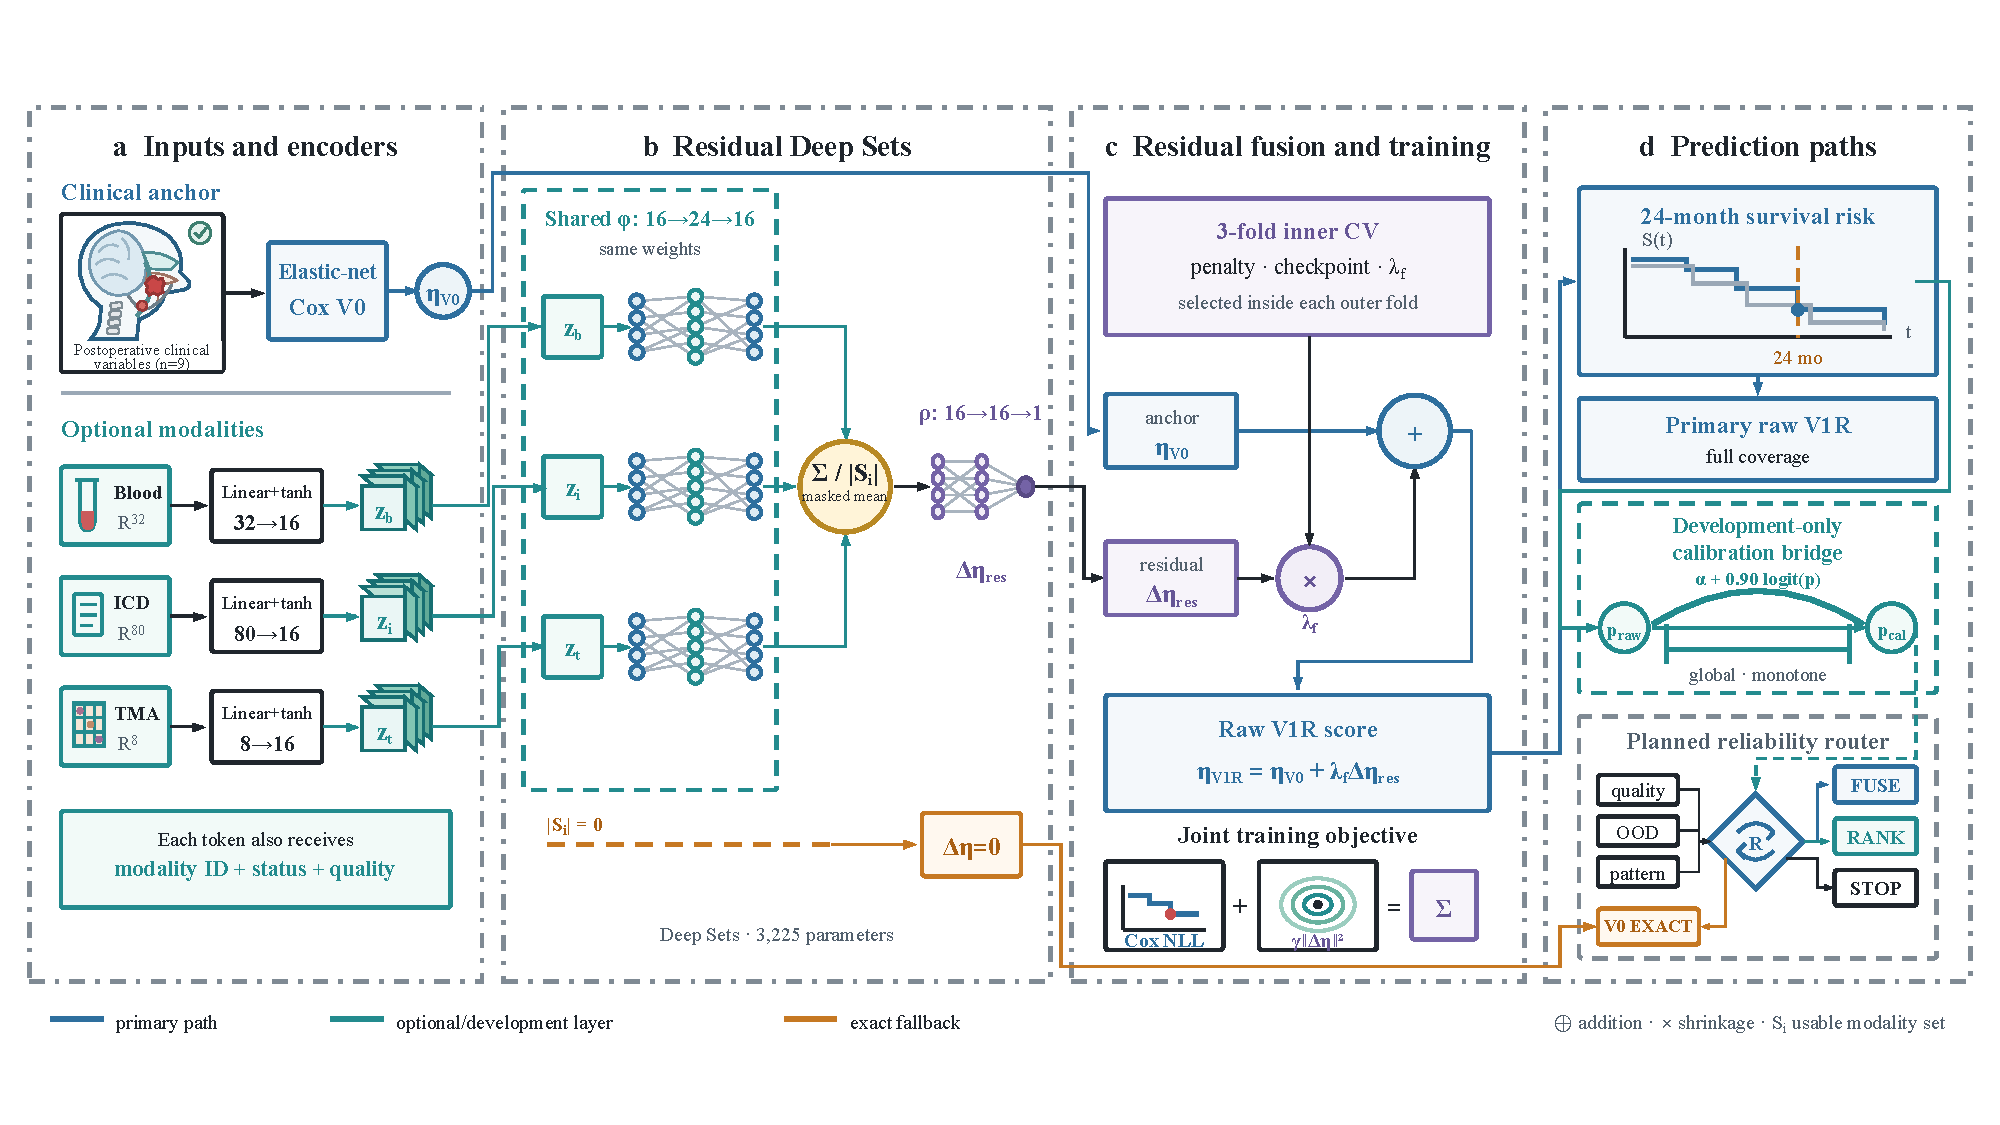
\includegraphics[width=\textwidth]{figures/figure1_pattern_surv_hn_framework.pdf}
\caption{\textbf{Clinically anchored residual fusion architecture for PATTERN-Surv-HN.} \textbf{a}, Postoperative clinical-pathological variables are encoded by an elastic-net Cox anchor (V0). \textbf{b}, Usable blood, ICD and TMA measurements are represented as unordered modality tokens with identity, availability/usability and quality indicators and processed by a shared permutation-invariant Deep Sets residual encoder. \textbf{c}, The residual is shrinkage-controlled and added to V0 to produce raw V1R; residual penalty, optimization checkpoint and fold-specific scale are selected in inner cross-validation. \textbf{d}, The primary prediction path is raw V1R with full coverage. If no optional modality is usable, the residual is zero and V0 is returned exactly. The global bridge is development-only; the reliability router is exploratory and not a validated deployment component.}\label{fig:architecture}
\end{figure*}

\begin{figure*}[t]
\centering
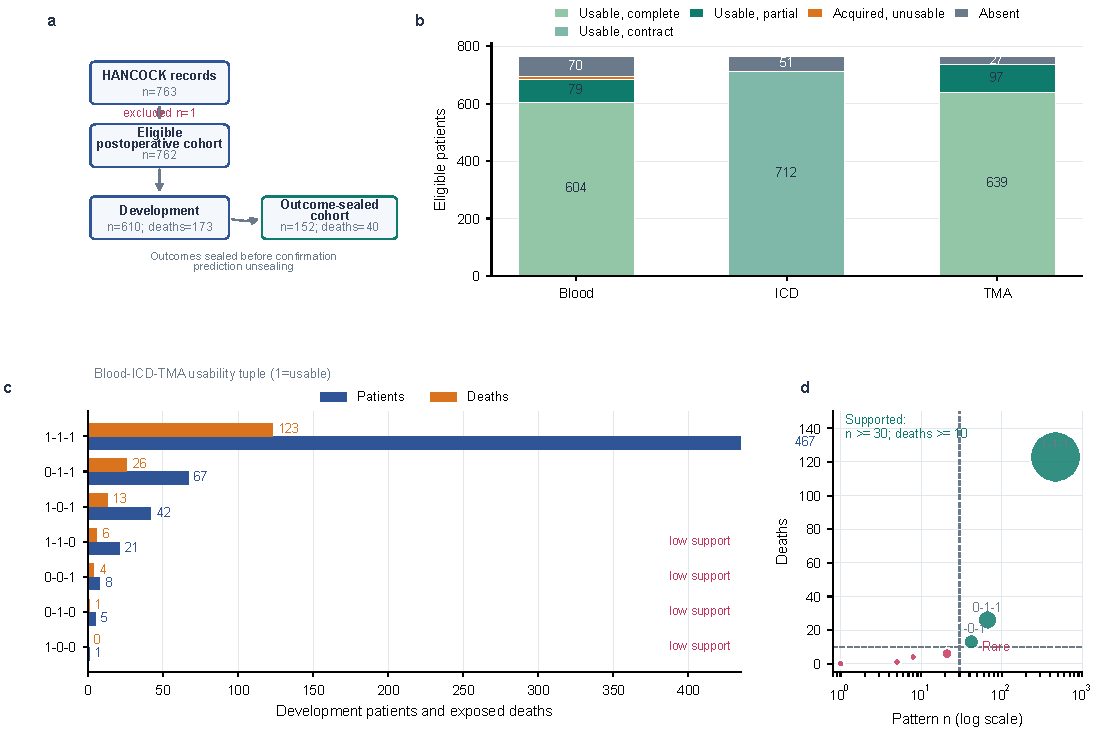
\includegraphics[width=\textwidth]{figures/figure2_cohort_flow_acquisition_usability.pdf}
\caption{\textbf{Cohort flow, acquisition, usability and pattern support in HANCOCK.} \textbf{a}, Records, exclusions, development cohort and outcome-sealed confirmation cohort. \textbf{b}, Eligible-patient status for blood, ICD and TMA; acquired-but-unusable inputs are distinguished from absent inputs. \textbf{c}, Development counts for blood--ICD--TMA usability tuples (1=usable); exposed deaths are shown only for non-sealed roles. \textbf{d}, Pattern support relative to the prespecified support threshold of at least 30 patients and 10 deaths. Rare patterns are descriptive and do not carry independent confirmatory support.}\label{fig:patterns}
\end{figure*}

\subsection{Shrinkage-controlled residual fusion improves development discrimination at full coverage}

V1R retained the clinical-pathological anchor V0 and added a residual learned only from usable optional modalities. Under five repetition seeds, five outer folds and three inner folds, mean 24-month Uno C increased from 0.644239 to 0.665542 (mean difference $+0.021303$), time-dependent AUC from 0.662022 to 0.682511 ($+0.020488$), and IPCW Brier score from 0.124745 to 0.124338 ($-0.000407$; Table~\ref{tab:development} and Fig.~\ref{fig:v1r}). The Uno C, AUC and Harrell C directions favoured V1R in all five seeds; IPCW Brier favoured V1R in three of five seeds.

The gain did not come from selective reporting. V0 and V1R both covered all 610 eligible development patients. When the usable optional set was empty, residual and fused-score fallback errors were exactly zero. The worst supported-pattern Brier regret was $+0.009848$, below the prespecified $+0.020$ no-harm boundary.

\begin{table*}[t]
\centering
\caption{Repeated nested development performance in HANCOCK}\label{tab:development}
\small\setlength{\tabcolsep}{3pt}
\begin{tabular}{lrrrrrr}
\toprule
Model & Brier$_{24}$ & Uno C$_{24}$ & AUC$_{24}$ & Harrell C & Coverage & Worst regret\\
\midrule
Clinical anchor (V0) & 0.124745 & 0.644239 & 0.662022 & 0.623021 & 100\% & reference\\
V1R residual fusion & 0.124338 & 0.665542 & 0.682511 & 0.633710 & 100\% & $+0.009848$\\
\bottomrule
\end{tabular}
\end{table*}

\begin{figure*}[t]
\centering
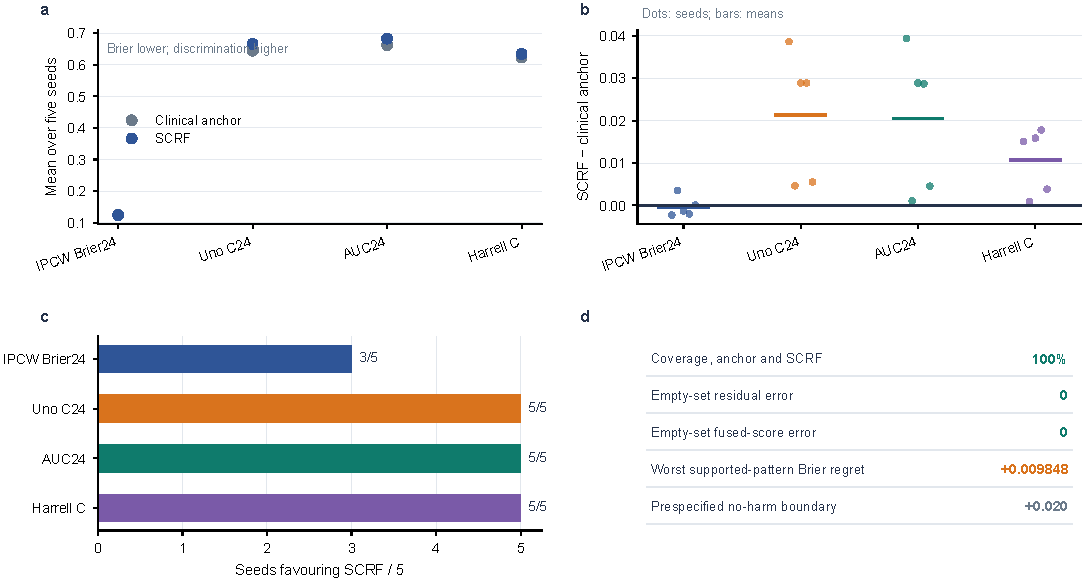
\includegraphics[width=\textwidth]{figures/figure3_v1r_development_performance_safety.pdf}
\caption{\textbf{V1R development performance, seed stability and full-coverage safety.} \textbf{a}, Five-seed mean performance for V0 and V1R. \textbf{b}, Seed-level paired differences (V1R$-$V0); horizontal bars are means. \textbf{c}, Number of seeds with a direction favouring V1R. \textbf{d}, Full-coverage and exact-empty-set fallback checks, with the worst supported-pattern Brier regret relative to the prespecified no-harm boundary. Evidence is development-only repeated nested cross-fitting, not external validation.}\label{fig:v1r}
\end{figure*}

\subsection{A rank-preserving bridge improves the development risk scale but does not transport}

Raw V1R showed mild under-dispersion in the development absolute-risk diagnostic (calibration slope 0.825887; calibration-in-the-large $+0.011680$). The separately evaluated U5R7 bridge used a fixed positive slope of 0.90 and a cross-fitted weighted-log-loss intercept on the logit scale. It preserved ranking and 100\% coverage while moving calibration-in-the-large to $-0.003796$ and slope to 0.881552 (Fig.~\ref{fig:bridge}). Its IPCW Brier penalty was $+0.000147$, within the development gate of $+0.0005$, and its worst supported-pattern regret was $+0.004176$, below $+0.005$.

U5R8 then applied the already frozen bridge without confirmation-cohort refitting, after the raw-V1R confirmation outcomes had been unsealed. Ranking and coverage remained preserved, but IPCW Brier worsened by $+0.001085$, absolute calibration-in-the-large error worsened by $+0.004194$, and absolute calibration-slope error worsened by $+0.167815$. Thus, the development calibration gain did not transport; the bridge remains development-only and is not a confirmed calibration layer.

\begin{figure*}[t]
\centering
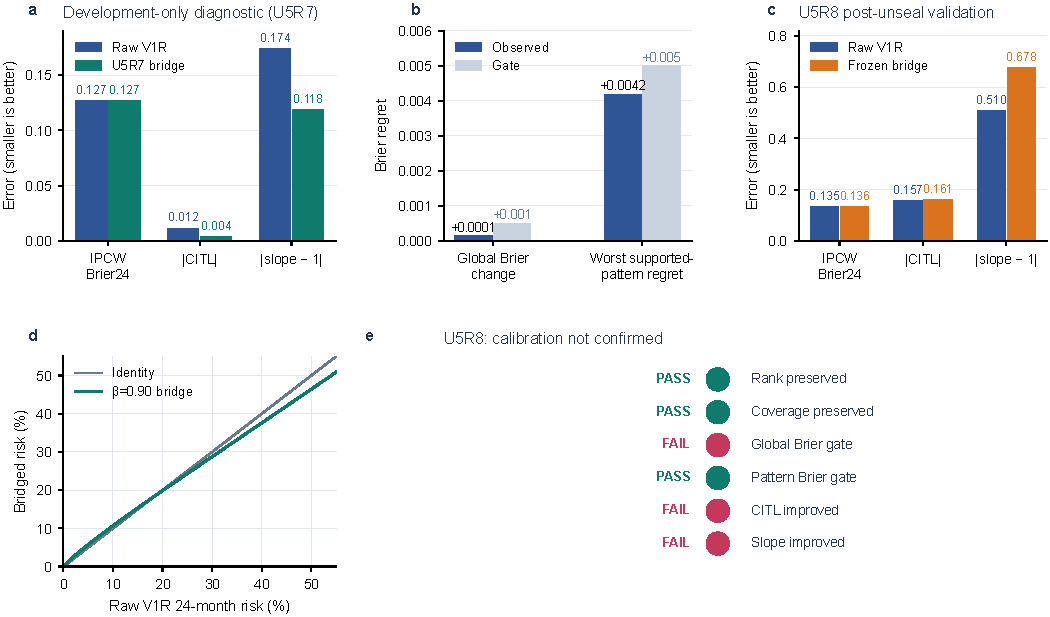
\includegraphics[width=\textwidth]{figures/figure4_calibration_bridge_development_and_transport.pdf}
\caption{\textbf{Development calibration bridge and locked secondary post-unseal validation.} \textbf{a}, U5R7 development-only absolute-risk errors for raw V1R and the bridge. \textbf{b}, Observed global and worst supported-pattern Brier regret relative to development gates. \textbf{c}, U5R8 comparison in the HANCOCK out-of-distribution cohort after raw-outcome unsealing. \textbf{d}, Fixed monotone bridge transformation. \textbf{e}, U5R8 safety and calibration checks. U5R7 is development-only; U5R8 failed calibration transport gates, so no confirmed calibration claim is made.}\label{fig:bridge}
\end{figure*}

\subsection{Locked outcome-untouched confirmation shows a favourable raw-V1R direction}

After the V1R protocol, input manifest, dependency lock and patient-level predictions had been frozen, confirmation outcomes were unsealed in 152 HANCOCK patients with 40 deaths. The primary readout was raw V1R, not the calibration bridge or router. V1R retained 100\% coverage and had favourable point estimates for Uno C (0.804242 versus 0.782579), IPCW Brier (0.131246 versus 0.136412), AUC$_{24}$ (0.813637 versus 0.801094) and Harrell C (0.752842 versus 0.733253; Table~\ref{tab:confirmation} and Fig.~\ref{fig:confirmation}).

Patient-level stratified bootstrap intervals crossed zero for every principal delta. For example, the mean delta Uno C was $+0.021654$ (95\% interval $-0.025965$ to $+0.070816$) and mean delta IPCW Brier was $-0.005222$ ($-0.012843$ to $+0.002171$). The locked result therefore supports a positive directional raw-V1R confirmation signal, not definitive superiority or clinical utility.

\begin{table*}[t]
\centering
\caption{Locked raw-V1R confirmation in the HANCOCK outcome-sealed cohort}\label{tab:confirmation}
\small\setlength{\tabcolsep}{3pt}
\begin{tabular}{lrrrr}
\toprule
Metric & V0 & Raw V1R & Difference & Bootstrap mean (95\% CI)\\
\midrule
Uno C$_{24}$ & 0.782579 & 0.804242 & $+0.021664$ & $+0.021654$ ($-0.025965$, $+0.070816$)\\
IPCW Brier$_{24}$ & 0.136412 & 0.131246 & $-0.005166$ & $-0.005222$ ($-0.012843$, $+0.002171$)\\
AUC$_{24}$ & 0.801094 & 0.813637 & $+0.012543$ & $+0.012725$ ($-0.041031$, $+0.068438$)\\
Harrell C & 0.733253 & 0.752842 & $+0.019589$ & $+0.019665$ ($-0.017423$, $+0.061196$)\\
Coverage & 100\% & 100\% & 0 & --\\
\bottomrule
\end{tabular}
\end{table*}

\begin{figure*}[t]
\centering
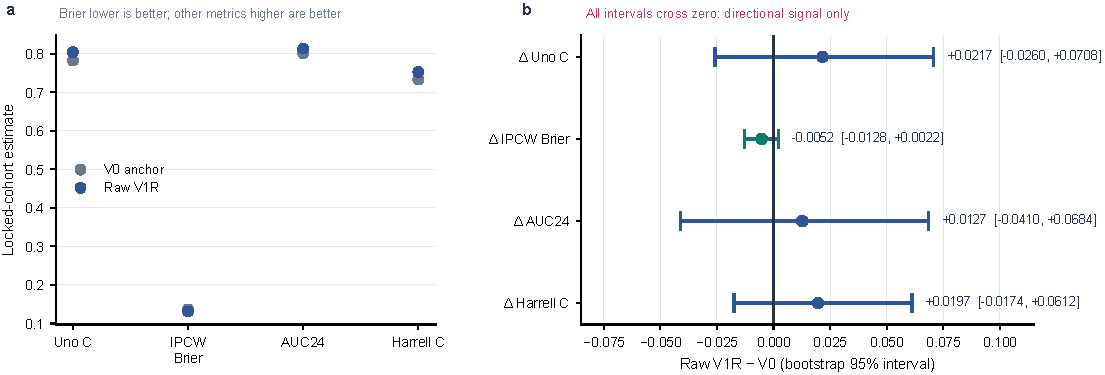
\includegraphics[width=\textwidth]{figures/figure5_locked_raw_v1r_confirmation.pdf}
\caption{\textbf{Locked outcome-untouched raw-V1R confirmation.} \textbf{a}, V0 and raw V1R point estimates in the HANCOCK confirmation cohort. \textbf{b}, Paired differences with patient-level stratified bootstrap 95\% intervals. All intervals cross zero; the result is a positive directional signal rather than proof of superiority.}\label{fig:confirmation}
\end{figure*}

\subsection{Exploratory extensions do not alter the confirmation boundary}

Several extensions were analysed after the core evidence and are reported separately. A cross-fitted patient-level value router selected raw V1R or V0 (Extended Data Fig.~1). Its best policy (reliability-augmented, threshold 0.60) reduced IPCW Brier versus V0 by 0.000506, but its bootstrap interval crossed zero and the router was worse than direct raw V1R while not preserving exact global ranking. An adapted clinical/radiomics characterization in RADCURE (626 patients, 110 events) showed strong descriptive performance for comparators C1--C4 (Extended Data Fig.~2), but RADCURE does not reproduce the frozen current blood--ICD--TMA contract and its outcomes had been consumed previously; it is not external validation of current V1R.

A transcriptome residual analogue, T1R, was then replicated in TCGA-HNSC (519 patients, 221 events; Extended Data Fig.~3). Mean IPCW Brier improved from 0.221795 to 0.218058 and Uno C from 0.565199 to 0.597265, satisfying the exploratory complexity gate. This is post-hoc method replication because TCGA outcomes had already been used. Descriptive application to GSE65858 and GSE41613 (Extended Data Fig.~4) showed favourable discrimination deltas but worse calibration in GSE65858; these GEO analyses are post-hoc characterization, not formal external validation.

\begin{figure*}[t]
\centering
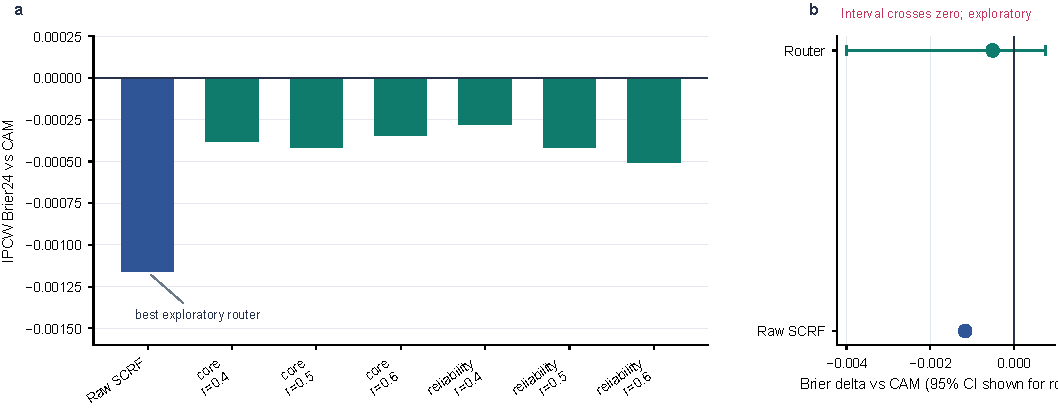
\includegraphics[width=\textwidth]{figures/extended_data_figure1_router_exploration.pdf}
\par\vspace{2pt}
{\raggedright\small\textbf{Extended Data Fig. 1 | Exploratory patient-level reliability router.} \textbf{a}, IPCW Brier differences versus V0 for raw V1R and router policies. \textbf{b}, Best router point estimate with bootstrap interval. All intervals crossed zero, the best router was worse than raw V1R, and global ranking was not exactly preserved; this is exploratory development analysis, not a validated deployment component.\par}
\end{figure*}

\begin{figure*}[t]
\centering
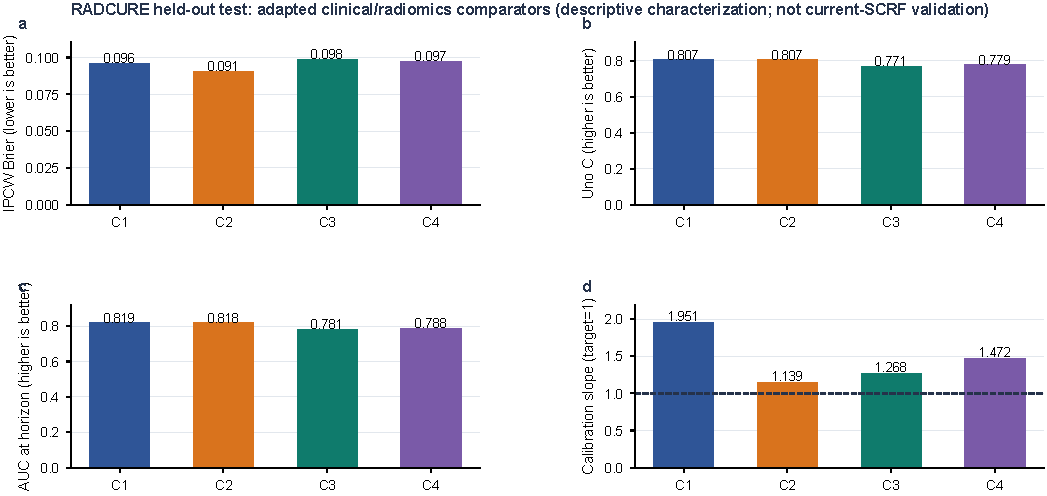
\includegraphics[width=\textwidth]{figures/extended_data_figure2_radcure_characterization.pdf}
\par\vspace{2pt}
{\raggedright\small\textbf{Extended Data Fig. 2 | RADCURE external characterization of adapted comparators.} \textbf{a--d}, IPCW Brier, Uno C, horizon AUC and calibration slope for adapted clinical/radiomics comparators C1--C4 in the held-out RADCURE test split. This descriptive analysis does not evaluate the frozen current blood--ICD--TMA V1R contract and is not current-V1R external validation.\par}
\end{figure*}

\begin{figure*}[t]
\centering
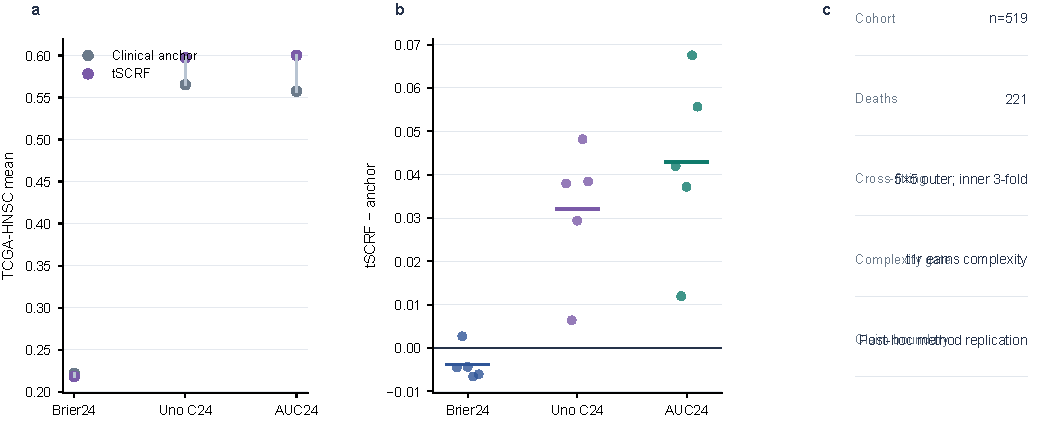
\includegraphics[width=\textwidth]{figures/extended_data_figure3_t1r_transcriptome_replication.pdf}
\par\vspace{2pt}
{\raggedright\small\textbf{Extended Data Fig. 3 | T1R transcriptome method replication in TCGA-HNSC.} \textbf{a}, Mean anchor and T1R performance. \textbf{b}, Seed-level T1R$-$anchor differences. \textbf{c}, Cohort and claim boundary. TCGA outcomes had already been consumed; therefore this is post-hoc method replication, not confirmatory validation.\par}
\end{figure*}

\begin{figure*}[t]
\centering
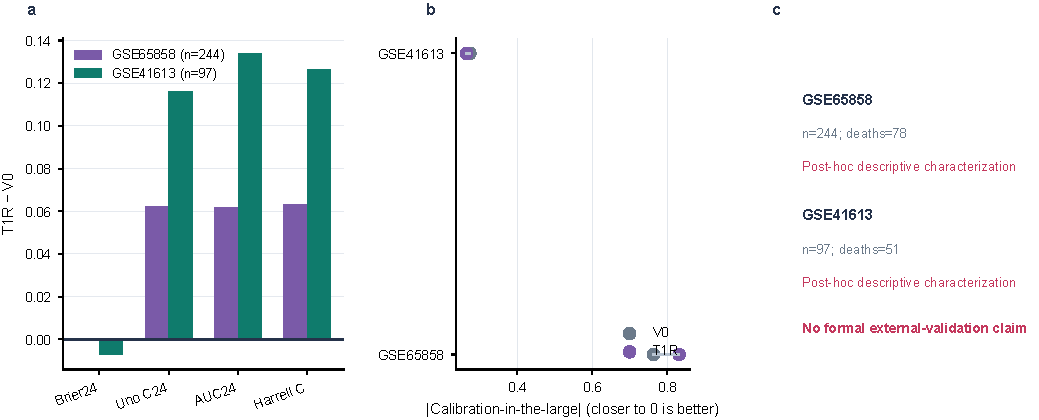
\includegraphics[width=\textwidth]{figures/extended_data_figure4_geo_t1r_characterization.pdf}
\par\vspace{2pt}
{\raggedright\small\textbf{Extended Data Fig. 4 | Post-hoc GEO characterization of T1R.} \textbf{a}, T1R$-$anchor differences in GSE65858 and GSE41613. \textbf{b}, Absolute calibration-in-the-large error. \textbf{c}, Cohort sizes and claim boundary. These are descriptive post-hoc analyses, not formal external validation.\par}
\end{figure*}

\section{Discussion}

The central finding is controlled incremental fusion. Optional blood, ICD and TMA measurements improved development discrimination when introduced as a shrinkage-controlled residual around a stable clinical-pathological anchor, while preserving full coverage and exact fallback. A positive-slope global bridge improved the development risk scale without changing patient ordering, coverage or fallback logic.

Development and locked confirmation tell a coherent but bounded story. V1R improved discrimination in every repetition seed and reduced primary probabilistic error in development. The separately evaluated bridge moved development calibration summaries toward their targets. In the outcome-untouched confirmation cohort, raw V1R again showed favourable point estimates, but bootstrap intervals crossed zero. The subsequent locked secondary U5R8 analysis showed that the fixed bridge did not reproduce its calibration gains. The appropriate interpretation is therefore a positive directional raw-V1R confirmation signal plus development-only bridge evidence---not proven superiority, confirmed absolute-risk transport, clinical utility or deployment readiness.

The result-informed development history makes V1R and U5R7 exploratory rather than preregistered confirmatory methods. Rare natural patterns have limited independent support, and the router, RADCURE, TCGA and GEO extensions do not alter the primary claim boundary. Future work should evaluate calibration transport in a genuinely independent cohort with the protocol frozen before outcome access, together with invalid-present controls, clinical utility, transportability and prospective implementation safeguards.

\section{Methods}

\subsection{Study design and reporting}
This retrospective, configuration-controlled modelling study separates development, calibration, locked confirmation and explicitly exploratory extension analyses. Reporting follows TRIPOD+AI principles, with PROBAST+AI-related risk-of-bias domains used to organize claim boundaries \cite{collins2024,moons2025}. Each analysis reports prior outcome access, cohort role, coverage, frozen artefact identity and whether a confirmatory claim is permitted.

\subsection{Cohorts and endpoint}
The primary ecosystem was HANCOCK \cite{dorrich2025}. After exclusions, 610 postoperative HNSCC patients (173 deaths) contributed to development and 152 patients (40 deaths) formed the outcome-sealed confirmation cohort. The endpoint was all-cause death, measured from first treatment to last information; the primary horizon was 730.5 days. Development used no confirmation outcomes. TCGA-HNSC, GSE65858, GSE41613 and RADCURE were used only in labelled post-hoc or descriptive extensions \cite{tcga2015,liu2018,wichmann2015,lohavanichbutr2013,welch2024}.

\subsection{Clinical anchor and V1R residual architecture}
V0 was an elastic-net Cox clinical-pathological anchor using age, sex, smoking, primary site, grade, p16, resection, pathological T and pathological N. Adjuvant treatment and post-prediction variables were excluded. Each usable blood, ICD or TMA measurement was represented as a token containing modality values, identity, usability/status and outcome-blind quality indicators. Tokens were pooled by a permutation-invariant masked-mean Deep Sets residual encoder. For patient $i$,
\begin{equation}
\eta_{\mathrm{V1R},i}=\eta_{\mathrm{V0},i}+\lambda_f g\left(\rho\left(\frac{1}{|S_i|}\sum_{m\in S_i}\phi(x_{im},q_{im},e_m)\right)\right),
\end{equation}
where $S_i$ is the usable optional-modality set, $x_{im}$ contains measurements, $q_{im}$ quality/status features, and $e_m$ a modality embedding. The model had 3,225 parameters. Residual penalty, optimization checkpoint and fold-specific residual scale $\lambda_f$ were selected only within three-fold inner cross-validation. Preprocessing and Breslow baseline estimation were fold-bound. When $S_i$ was empty, the residual was exactly zero and the prediction equalled V0.

\subsection{Development calibration bridge}
For each held-out outer fold, the raw V1R 24-month risk was transformed by
\begin{align}
x_{\mathrm{raw},i}&=\operatorname{logit}(p_{\mathrm{V1R},i}),\\
x_{\mathrm{bridge},i}&=\alpha_{\mathrm{logloss},f}+0.90x_{\mathrm{raw},i},\qquad p_{\mathrm{bridge},i}=\sigma(x_{\mathrm{bridge},i}).
\end{align}
The intercept was fitted by weighted log-loss using non-held-out development folds only. The bridge was global, strictly monotone and used no pattern-specific adjustment. The development diagnostic used five seeds, five outer folds, 2,460 repeated out-of-fold rows and 415 evaluable events. Gates were global Brier change $\leq +0.0005$, worst supported-pattern regret $\leq +0.005$, CITL and slope improvement, ranking preservation and full coverage.

\subsection{Locked confirmation and secondary bridge validation}
The confirmation protocol, input manifest, dependency lock and prediction artefact were frozen before outcomes were unsealed. Twenty-five matched V0/V1R members (five seeds by five outer folds) were generated with development-fold fitting only and no confirmation tuning, bridge, router, refitting or patient removal. Confirmation outcomes were read after prediction sealing. Aggregate uncertainty used 2,000 patient-level stratified bootstrap replicates (seed 20260825). The primary confirmation readout was raw V1R. U5R8 separately reused the frozen $\beta=0.90$ bridge with the arithmetic mean development intercept ($\alpha=-0.1450338$), using 2,000 event-stratified replicates (seed 20260827). Because U5R8 occurred after raw-outcome unsealing, it is explicitly a locked secondary post-unseal validation.

\subsection{Exploratory extensions}
The U6R1 router used cross-fitted patient-level value estimates and reliability proxies to choose raw V1R or V0; 2,000 bootstrap replicates quantified uncertainty. U7R2 evaluated adapted clinical/radiomics comparators C1--C4 on the RADCURE held-out test split. U8 replicated the residual-shrinkage architecture with transcriptome tokens in previously consumed TCGA-HNSC data. U8E applied a single full-development T1R fit to GSE65858 and GSE41613 without external refitting. None of these analyses permits a current-V1R confirmatory or external-validation claim.

\subsection{Estimands and metrics}
Paired development and confirmation estimands were $\Delta\mathrm{Brier}_{24}=\mathrm{Brier}_{24}(\mathrm{V1R})-\mathrm{Brier}_{24}(\mathrm{V0})$ and analogous discrimination deltas. Lower Brier and higher discrimination values are better. Calibration-in-the-large (CITL) is better closer to zero; calibration slope is better closer to one. Pattern safety used
\begin{equation}
\mathcal{R}_{\mathrm{worst}}=\max_{p\in\mathcal{P}_{\mathrm{supported}}}\{\mathrm{Brier}_{24}(\mathrm{bridge},p)-\mathrm{Brier}_{24}(\mathrm{V1R},p)\},
\end{equation}
with supported patterns requiring at least 30 patients and 10 events. IPCW weighting addressed censoring; Uno C, horizon AUC and Harrell C summarized ranking.

\subsection{Reproducibility and governance}
Repetition seeds were 17, 29, 43, 71 and 101. All result figures and tables were generated from aggregate JSON artefacts; no patient-level predictions are included in the manuscript repository. Development out-of-fold, locked-protocol and sealed-prediction SHA256 values are retained in the aggregate provenance files and figure manifest. Figure provenance is recorded in \texttt{figures/figure\_manifest.json}; figure generation uses \texttt{generate\_figures.py}. A large-language-model-assisted coding and writing tool helped organize code, wording and LaTeX; it was not an author and did not independently generate or validate results. Final author verification is required.

\subsection{Ethics}
This analysis used retrospective datasets under their original governance and access conditions; no participants were newly recruited. Dataset-specific review-board approval, consent/waiver language, accessions, versions and secondary-analysis exemptions remain to be reproduced before submission. No patient/public involvement has been documented.

\section*{Data availability}
HANCOCK, TCGA-HNSC, GSE65858, GSE41613 and RADCURE are available subject to source conditions \cite{dorrich2025,tcga2015,wichmann2015,lohavanichbutr2013,welch2024}. The repository tracks aggregate metrics, frozen specifications, audits and figure-generation code. Patient-level predictions remain outside version control and will not be redistributed contrary to source terms. \TBD{Add final accession/version table and archival DOI.}

\section*{Code availability}
The configuration-driven \texttt{trust-hn} repository contains model code, frozen contracts, aggregate audits and tests. \TBD{Add public archival release, licence, environment lock and runtime details.}

\section*{Acknowledgements}
\TBD{Funding, data contributors, collaborators and computing resources.}

\section*{Author contributions}
\TBD{Complete CRediT roles for all authors.}

\section*{Competing interests}
The authors declare \TBD{no competing interests / specify}.

\section*{Additional information}
\textbf{Supplementary information:} the Supplementary Information provides Supplementary Note~1, expanded Supplementary Methods and Results, and Supplementary Tables~1--8 covering V1R development, calibration bridging, locked confirmation, reliability-aware routing, RADCURE benchmarking, TCGA method replication and GEO cross-platform characterization. The completed TRIPOD+AI checklist and PROBAST+AI assessment will accompany the submission package.\\
\textbf{Extended Data:} Extended Data Figs. 1--4 report exploratory router, RADCURE, TCGA and GEO analyses.\\
\textbf{Correspondence:} \TBD{corresponding author}.\\
\textbf{Provenance and peer review:} \TBD{journal completion}.

\bibliography{references}
\end{document}


